% 7. Accepttest
\chapter{Accepttest}

\begin{table}[!htbp] \centering
\begin{tabular}{|p{2cm}|p{8cm}|}
	\hline
		\multicolumn{2}{|l|}{Versionshistorik} \\\hline
		\textbf{v1.0} &15-03-2016 Pre-review\\\hline
	\end{tabular}
\end{table}

Punkterne i Accepttestspecifikationen, er skrevet ud fra punkterne i hovedforløbet, for de enkelte usecases.

\section{Testopstilling}

\begin{figure}[H]
\centering
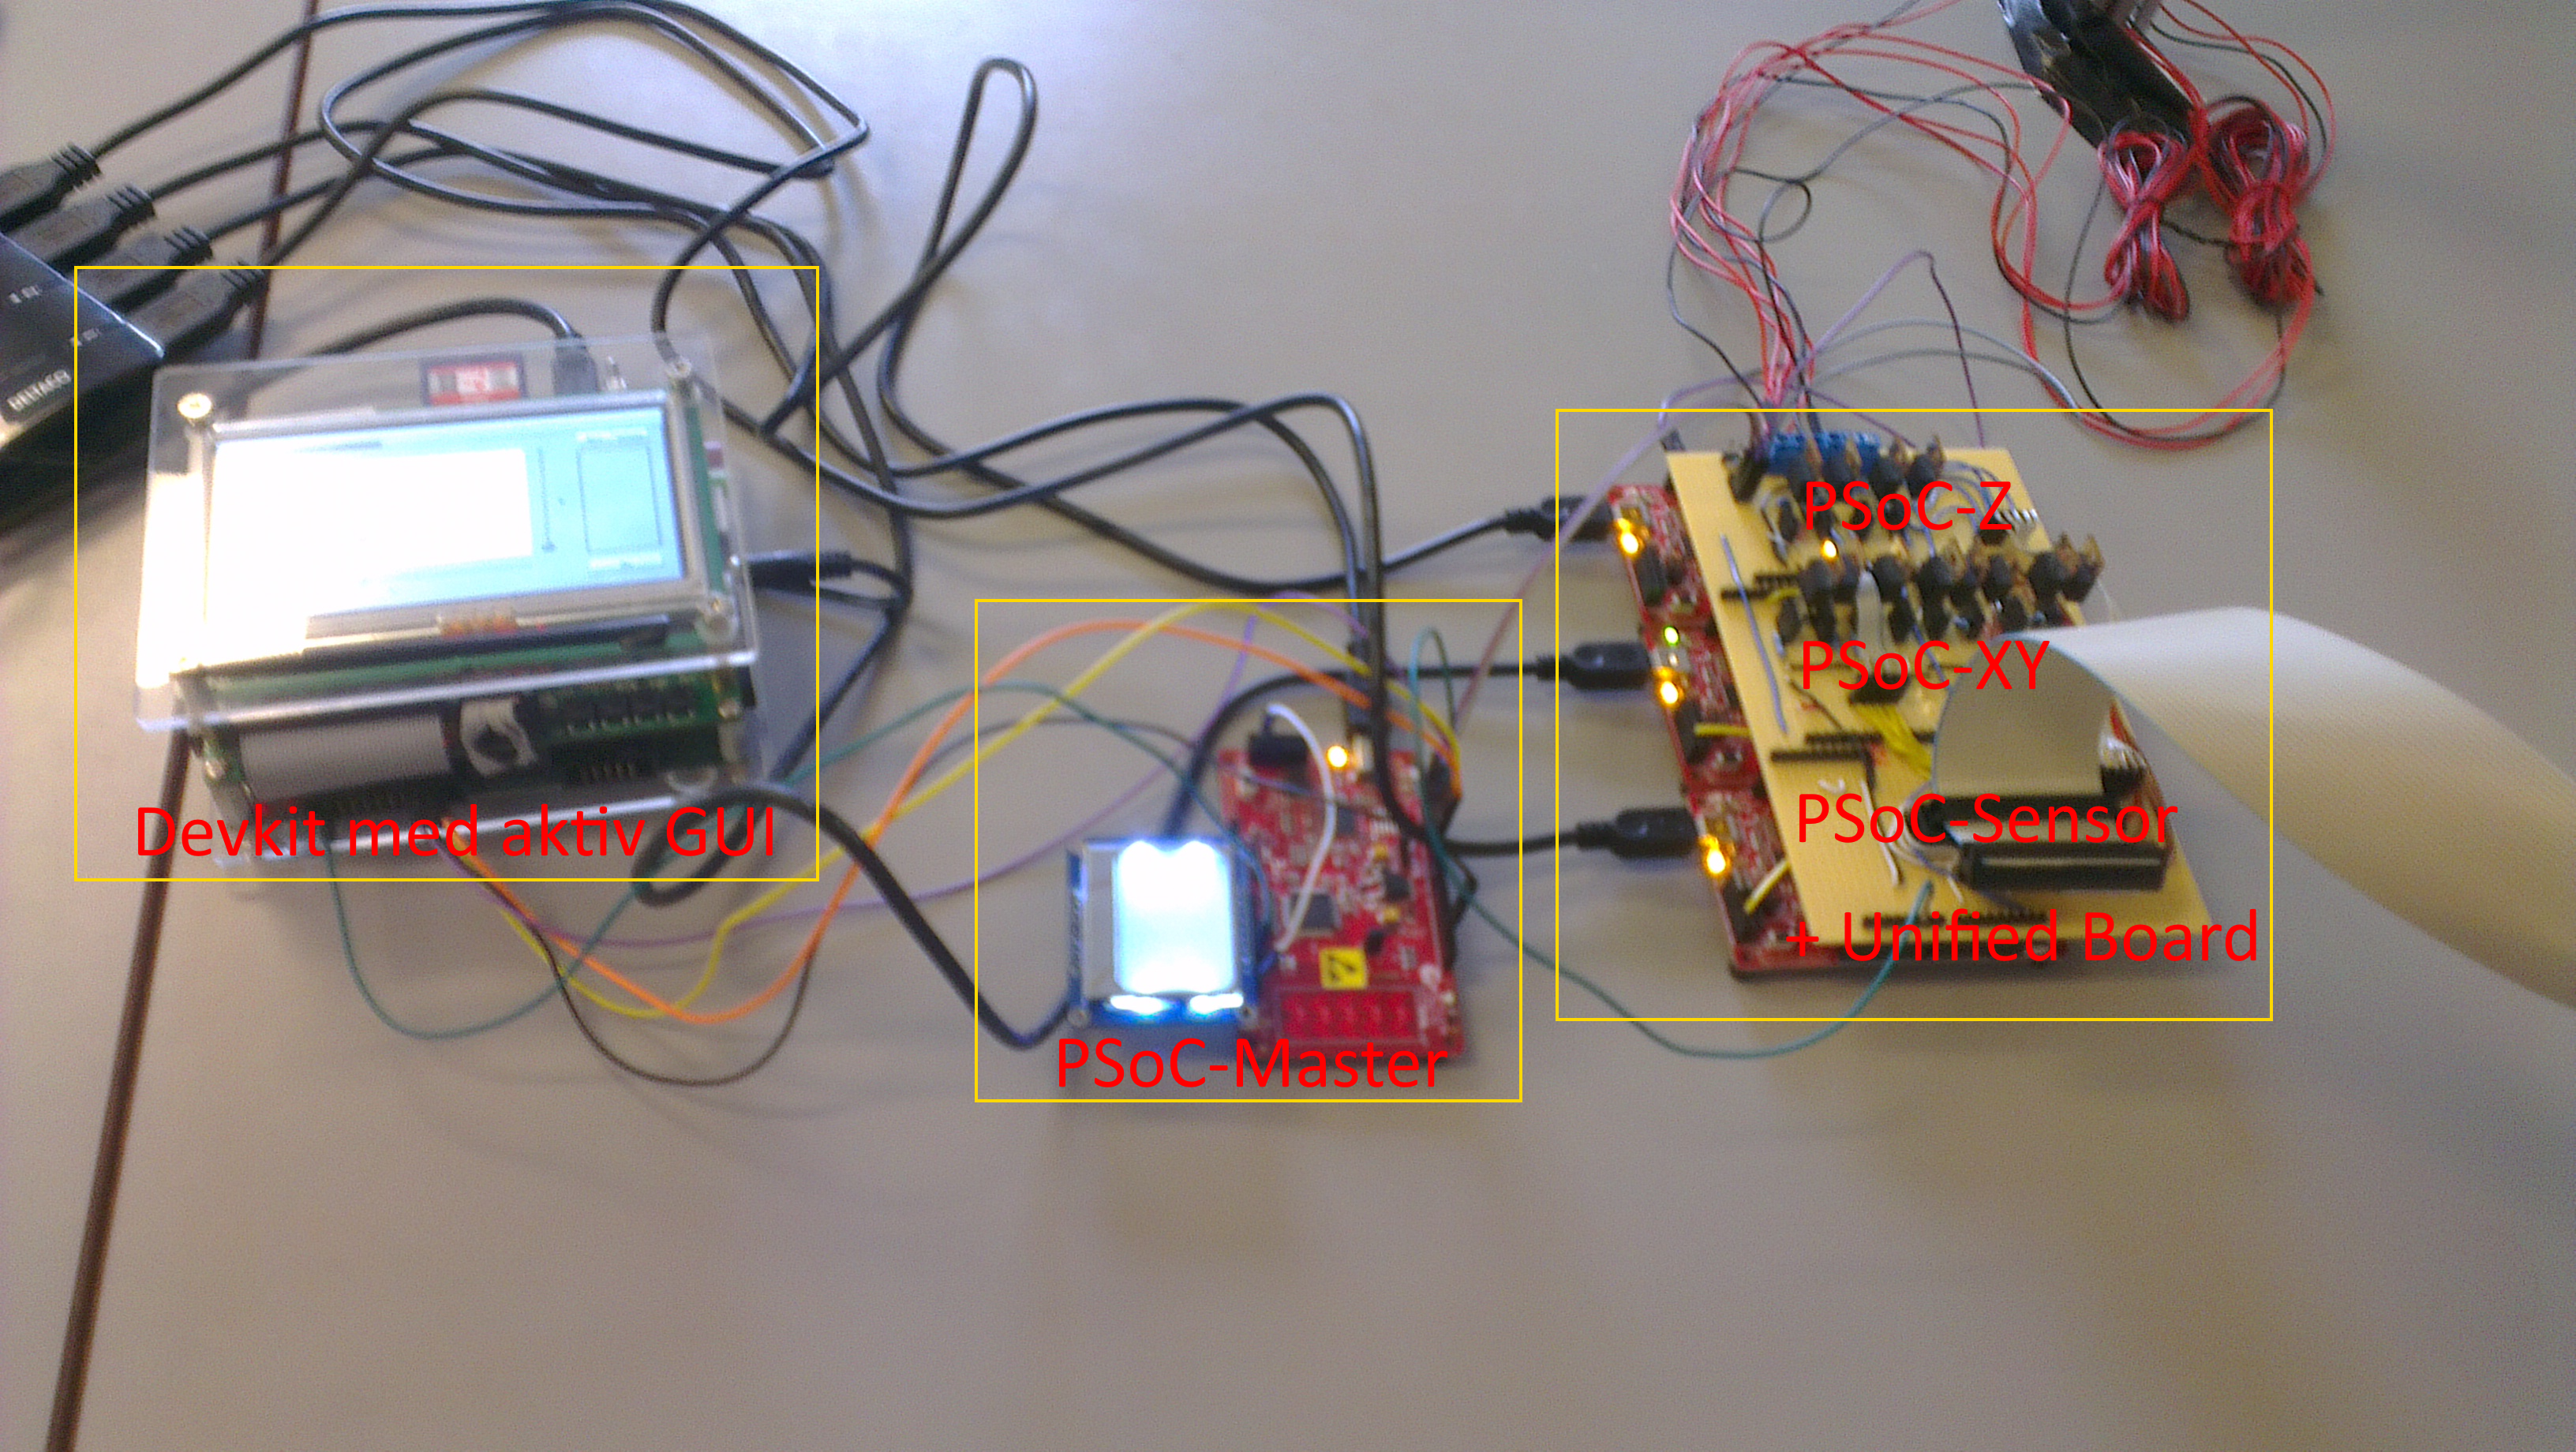
\includegraphics[width=1.0\linewidth]{0_Filer/Figuer/testopstilling.png}
\caption{Testopstillingsbillede}
\label{fig:testopstilling}
\end{figure}

En tændt computer med Teraterm åbent tilsluttes med USB til PSoC Master for at kontrollere at kommunikationen igennem hele systemet forløber korrekt. Et Devkit8000 med GUI’en aktivt kørende tilsluttes med de korrekte ledningsforbindelser til PSoC Master. Devkit8000 tilkobles en PC koblet på Devkittet til aflæsning af qDebug returværdier. På PSoC Masteren tilsluttes et Nokia 5150 display til udskrivning af modtaget beskeder til postkontoret. Til PSoC Masteren tilkobles de tre PSoC slaver: PSoC Z, PSoC XY og PSoC Sensor i nævnte rækkefølge fra venstre mod højre og alle tre monteret Unified Board som anvist på testopstillingsbilledet. Ledningsforbindelserne fra Unified Board tilsluttes til resten af systemet med ledninger og fladkabel.

% Accepttest Use Case 1
\section{ATUC1: Kalibrér system}

\begin{center} \centering
    \begin{longtable}{|p{0,5cm}|p{3,7cm}|p{3,7cm}|p{2,3cm}|p{2,3cm}|}
    \hline
        \multicolumn{5}{|l|}{\textbf{ATUC1: Kalibrer system}} \\ \hline
        \multicolumn{1}{|c|}{} &
        \textbf{Test} &
        \textbf{Forventet \newline Resultat} &
        \textbf{Resultat} &
        \textbf{Godkendt\slash \newline Kommentar} \\ \hline 
        \endfirsthead

        \multicolumn{5}{l}{...fortsat fra forrige side} \\ \hline 
        \multicolumn{5}{|l|}{\textbf{ATUC1: Kalibrer system}} \\ \hline
        \multicolumn{1}{|c|}{} &
        \textbf{Test} &
        \textbf{Forventet \newline Resultat} &
        \textbf{Resultat} &
        \textbf{Godkendt\slash \newline Kommentar} \\ \hline 
        \endhead
        
        \multicolumn{5}{r}{fortsættes på næste side...} \\
        \endfoot
        \endlastfoot

        \textbf{1} 
            & Brugeren trykker ”Calibrate”-knap på touchskærmen under Settings-tabben.
            & Lampen trækkes helt op og bliver så kørt helt frem og tilbage i først X-dimensionen og dernæst Y-dimensionen. Disse kalibreringsværdier forventes returneret og gemt til de pågældende PSoC'er.
            & Kalibreringsrutinen blev tilendebragt i alle tre akser fejlfrit og kalibreringsdata blev gemt.	
            & Godkendt. 
        \\ \hline
	\end{longtable}
	\label{ATUC1} 
\end{center}

% Accepttest Use Case 2
\section{ATUC2: Tænd/sluk lys}

\begin{center} \centering
    \begin{longtable}{|p{0,5cm}|p{3,7cm}|p{3,7cm}|p{2,3cm}|p{2,3cm}|}
    \hline
        \multicolumn{5}{|l|}{\textbf{ATUC2: Tænd/sluk lys}} \\ \hline
        \multicolumn{1}{|c|}{} &
        \textbf{Test} &
        \textbf{Forventet \newline Resultat} &
        \textbf{Resultat} &
        \textbf{Godkendt\slash \newline Kommentar} \\ \hline 
        \endfirsthead

        \multicolumn{5}{l}{...fortsat fra forrige side} \\ \hline 
        \multicolumn{5}{|l|}{\textbf{ATUC2: Tænd/sluk lys}} \\ \hline
        \multicolumn{1}{|c|}{} &
        \textbf{Test} &
        \textbf{Forventet \newline Resultat} &
        \textbf{Resultat} &
        \textbf{Godkendt\slash \newline Kommentar} \\ \hline 
        \endhead

        \multicolumn{5}{r}{fortsættes på næste side...} \\
        \endfoot
        \endlastfoot
        
        \textbf{1} 
            & Brugeren indstiller en tilfældig farve med R-, G- og B-sliderne i Light-tabben.
            & Lyspaletten på touchskærmen opdateres til en farve i overensstemmelse med de indstillede sliderværdier.
            & Lyspaletten blev opdateret til valgte værdig
            &  Godkendt.
        \\ \hline
        \textbf{2} 
            & Brugeren trykker på Go-knappen placeret under R-, G- og B-sliderne.
            & Lampens lys bliver sat til den samme farve som den fremviste på touchskærmen.
            & Lampens lys stemte overens med farvepaletten.
            & Godkendt.
        \\ \hline
        \textbf{3} 
            & Brugeren trykker på ”On/Off”-knap på touchskærmen under Light-tabben på touchskærmen.
            & Lyset skifter tilstand, fra tændt til slukket, eller fra slukket til tændt med valgte sliderfarve.
            & Lyset slukkede ved tryk på Off-knappen og tændte igen ved tryk på On-knappen.
            & Godkendt.
        \\ \hline
	\end{longtable}
	\label{ATUC2}
\end{center}

% Accepttest Use Case 3
\section{ATUC3: Registrér bevægelse}

\begin{center} \centering
    \begin{longtable}{|p{0,5cm}|p{3,7cm}|p{3,7cm}|p{2,3cm}|p{2,3cm}|}
    \hline
        \multicolumn{5}{|l|}{\textbf{ATUC3: Registrér bevægelse}} \\ \hline
        \multicolumn{1}{|c|}{} &
        \textbf{Test} &
        \textbf{Forventet \newline Resultat} &
        \textbf{Resultat} &
        \textbf{Godkendt\slash \newline Kommentar} \\ \hline 
        \endfirsthead

        \multicolumn{5}{l}{...fortsat fra forrige side} \\ \hline 
        \multicolumn{5}{|l|}{\textbf{ATUC3: Registrér bevægelse}} \\ \hline
        \multicolumn{1}{|c|}{} &
        \textbf{Test} &
        \textbf{Forventet \newline Resultat} &
        \textbf{Resultat} &
        \textbf{Godkendt\slash \newline Kommentar} \\ \hline 
        \endhead

        \multicolumn{5}{r}{fortsættes på næste side...} \\
        \endfoot
        \endlastfoot
        
        \textbf{1} 
            & Bruger sætter Movement detection slideren til On på touchdisplayet under Sensor-tabben.
            & Slideren skifter position til On-positionen og bliver grøn.
            & Slideren skiftede til korrekt position og farve.	
            & Godkendt.
        \\ \hline
        \textbf{2} 
            & Bruger fører en arm forbi bevægelsessensoren på en afstand mindre end den fastsatte værdi under "Distance limit" spinboxen på touch displayet's Sensor-tab.
            & Lyset tændes med samme farve som angivet på Light-tabbens farvepalette på touchskærmen.
            & Lyset blev tændt med den samme værdi som den valgte Light-tabben.	
            & Godkendt. 
        \\ \hline
	\end{longtable}
	\label{ATUC3}
\end{center}

% Accepttest Use Case 4
\section{ATUC4: Justér lysets farve }

\begin{center} \centering
    \begin{longtable}{|p{0,5cm}|p{3,7cm}|p{3,7cm}|p{2,3cm}|p{2,3cm}|}
    \hline
        \multicolumn{5}{|l|}{\textbf{ATUC4: Justér lysets farve }} \\ \hline
        \multicolumn{1}{|c|}{} &
        \textbf{Test} &
        \textbf{Forventet \newline Resultat} &
        \textbf{Resultat} &
        \textbf{Godkendt\slash \newline Kommentar} \\ \hline 
        \endfirsthead

        \multicolumn{5}{l}{...fortsat fra forrige side} \\ \hline 
        \multicolumn{5}{|l|}{\textbf{ATUC4: Justér lysets farve }} \\ \hline
        \multicolumn{1}{|c|}{} &
        \textbf{Test} &
        \textbf{Forventet \newline Resultat} &
        \textbf{Resultat} &
        \textbf{Godkendt\slash \newline Kommentar} \\ \hline 
        \endhead

        \multicolumn{5}{r}{fortsættes på næste side...} \\
        \endfoot
        \endlastfoot
        
        \textbf{1} 
            & Brugeren sætter fingeren på rød farve-slideren "R"  på touchskærmen.
            & Slideren følger fingeren op og ned.
            & Slideren følger fingeren op og ned på "R"slideren.	
            &  Godkendt.
        \\ \hline
        \textbf{2} 
            & Brugeren trækker slideren helt til minimum (0) og trykker dernæst på Go-knappen under farvesliderne.
            & Den korresponderende farve i lampens diode slukkes helt.
            & Farven i lampens diode dæmpes for rød. 	
            & Godkendt.
        \\ \hline
        \textbf{3} 
            & Brugeren trækker slideren helt til maximum (255) og trykker dernæst på Go-knappen under farvesliderne.
            & Den korresponderende farve i lampens diode forstærkes til maksimal lysstyrke.
            & Farven i lampens diode forstærkes for rød.	
            & Godkendt.
        \\ \hline
        \textbf{4} 
            & Brugeren gentager trin 1 til 3 med grøn farve-slideren "G" og blå farve-slideren "B".
            & Samme resultater forventes for alle farver.
            & Samme resultat ses for alle tre farver.	
            & Godkendt.
        \\ \hline
	\end{longtable}
	\label{ATUC4}
\end{center}

% Accepttest Use Case 5
\section{ATUC5: Indstil placering af lampen}

\begin{center} \centering
    \begin{longtable}{|p{0,5cm}|p{3,7cm}|p{3,7cm}|p{2,3cm}|p{2,3cm}|}
    \hline
        \multicolumn{5}{|l|}{\textbf{ATUC5: Indstil placering i loft}} \\ \hline
        \multicolumn{1}{|c|}{} &
        \textbf{Test} &
        \textbf{Forventet \newline Resultat} &
        \textbf{Resultat} &
        \textbf{Godkendt\slash \newline Kommentar} \\ \hline 
        \endfirsthead

        \multicolumn{5}{l}{...fortsat fra forrige side} \\ \hline 
        \multicolumn{5}{|l|}{\textbf{ATUC5: Indstil placering i loft}} \\ \hline
        \multicolumn{1}{|c|}{} &
        \textbf{Test} &
        \textbf{Forventet \newline Resultat} &
        \textbf{Resultat} &
        \textbf{Godkendt\slash \newline Kommentar} \\ \hline 
        \endhead

        \multicolumn{5}{r}{fortsættes på næste side...} \\
        \endfoot
        \endlastfoot
        
        \textbf{1} 
            & Brugeren trækker i Y-slideren i opadgående retning på touchskærmens Position-tab.
            & Det røde ikon på touchskærmens Position-tab bevæger sig i opadgående retning og Y-sliderens tilhørende talværdi opdateres til en højere talværdi en den forhenværende.
            & Det røde ikon bevægede sig opad i takt med at Y-slideren bevægede sig opad. Talværdien blev opdateret til en forøget værdi.
            & Godkendt.
        \\ \hline
        \textbf{2} 
            & Brugeren trækker i Y-slideren i nedadgående retning på touchskærmens Position-tab.
            & Det røde ikon på touchskærmens Position-tab bevæger sig i opadgående retning og Y-sliderens tilhørende talværdi opdateres til en lavere talværdi en den forhenværende.
            & Det røde ikon bevægede sig nedad i takt med at Y-slideren bevægede sig opad. Talværdien blev opdateret til en formindsket værdi.
            & Godkendt.
        \\ \hline
        \textbf{3} 
            & Brugeren trækker i X-slideren i retningen mod højre på touchskærmens Position-tab.
            & Det røde ikon på touchskærmens Position-tab bevæger sig i retningen mod højre og X-sliderens tilhørende talværdi opdateres til en højere talværdi en den forhenværende.
            & Det røde ikon bevægede sig mod højre i takt med at X-slideren bevægede sig mod højre. Talværdien blev opdateret til en forøget værdi.
            & Godkendt
        \\ \hline
        \textbf{4} 
            & Brugeren trækker i X-slideren i retningen mod venstre på touchskærmens Position-tab.
            & Det røde ikon på touchskærmens Position-tab bevæger sig i retningen mod venstre og X-sliderens tilhørende talværdi opdateres til en lavere talværdi en den forhenværende.
            & Det røde ikon bevægede sig mod højre i takt med at X-slideren bevægede sig mod højre. Talværdien blev opdateret til en formindsket værdi.	
            & Godkendt 
        \\ \hline
        \textbf{5} 
            & Brugeren trækker i Z-slideren i opadgående retning på touchskærmens Position-tab.
            & Z-sliderens tilhørende talværdi opdateres til en højere talværdi en den forhenværende.
            & Talværdien blev opdateret til en forøget værdi.	
            & Godkendt. 
        \\ \hline
        \textbf{6} 
            & Brugeren trækker i Z-slideren i nedadgående retning på touchskærmens Position-tab.
            & Z-sliderens tilhørende talværdi opdateres til en lavere talværdi en den forhenværende.
            & Talværdien blev opdateret til en formindsket værdi.
            & Godkendt. 
        \\ \hline
        \textbf{7} 
            & Brugeren trykker på Go-knappen på touchskærmens Position-tab.
            & Et grønt ikon dækker det røde ikon og lampen bevæger sig nu afhængigt af de nu valgte sliderpositioner for X, Y og Z.
            & Et grønt ikon dækkede det røde ikon og lampen bevægede sig afhængigt af de valgte X-, Y- og Z-værdier.	
            & Godkendt. 
        \\ \hline
	\end{longtable}
	\label{ATUC5}
\end{center}

% Accepttest Use Case 6
\input{7_Accepttest/atuc6}

% Accepttest Use Case 7
\input{7_Accepttest/atuc7}

% Accepttest Use Case 8
%\section{ATUC8: Tilføj plan}

\begin{center} \centering
    \begin{longtable}{|p{0,5cm}|p{3,7cm}|p{3,7cm}|p{2,3cm}|p{2,3cm}|}
    \hline
        \multicolumn{5}{|l|}{\textbf{ATUC8: Tilføj plan}} \\ \hline
        \multicolumn{1}{|c|}{} &
        \textbf{Test} &
        \textbf{Forventet \newline Resultat} &
        \textbf{Resultat} &
        \textbf{Godkendt\slash \newline Kommentar} \\ \hline 
        \endfirsthead

        \multicolumn{5}{l}{...fortsat fra forrige side} \\ \hline
        \multicolumn{5}{|l|}{\textbf{ATUC8: Tilføj plan}} \\ \hline
        \multicolumn{1}{|c|}{} &
        \textbf{Test} &
        \textbf{Forventet \newline Resultat} &
        \textbf{Resultat} &
        \textbf{Godkendt\slash \newline Kommentar} \\ \hline 
        \endhead

        \multicolumn{5}{r}{fortsættes på næste side...} \\
        \endfoot
        \endlastfoot
        
        \textbf{1} 
            & Brugeren klikker ”Planner” fanen på Devkit8000-touchskærmen.
            & ”Planner” fanen vises på Devkit8000-touchskærmen. 
            & 	
            &  
        \\ \hline
        \textbf{2} 
            & Brugeren klikker på ”Save location”-knappen på Devkit8000-touchskærmen.
            & Devkit8000-touchskærmen beder brugeren om at indtaste et navn.
            & 	
            &  
        \\ \hline
        \textbf{3} 
            & Brugeren indtaster et navn på 10 tegn og trykker på ”Save” knappen
            & Systemet giver besked om at positionen er gemt i systemet. 
            & 	
            &  
        \\ \hline
	\end{longtable}
	\label{ATUC8}
\end{center}

% Accepttest Use Case 9
%\section{ATUC9: Vælg plan}

\begin{center} \centering
    \begin{longtable}{|p{0,5cm}|p{3,7cm}|p{3,7cm}|p{2,3cm}|p{2,3cm}|}
    \hline
        \multicolumn{5}{|l|}{\textbf{ATUC9: Vælg plan}} \\ \hline
        \multicolumn{1}{|c|}{} &
        \textbf{Test} &
        \textbf{Forventet \newline Resultat} &
        \textbf{Resultat} &
        \textbf{Godkendt\slash \newline Kommentar} \\ \hline 
        \endfirsthead

        \multicolumn{5}{l}{...fortsat fra forrige side} \\ \hline 
        \multicolumn{5}{|l|}{\textbf{ATUC9: Vælg plan}} \\ \hline
        \multicolumn{1}{|c|}{} &
        \textbf{Test} &
        \textbf{Forventet \newline Resultat} &
        \textbf{Resultat} &
        \textbf{Godkendt\slash \newline Kommentar} \\ \hline 
        \endhead

        \multicolumn{5}{r}{fortsættes på næste side...} \\
        \endfoot
        \endlastfoot
        
        \textbf{1} 
            & Brugeren klikker på ”Planner” fanen på Devkit8000-touchskærmen.
            & ”Planner” fanen vises på Devkit8000-touchskærmen.
            & 	
            &  
        \\ \hline
        \textbf{2} 
            & Brugeren klikker på en gemt plan på Devkit8000-touchskærmen.
            & En meddelelse om at en plan er valgt vises på Devkit8000-touchskærmen.
            & 	
            &  
        \\ \hline
	\end{longtable}
	\label{ATUC9}
\end{center}